%-----------------------------------------------
% Template para criação de resumos de projectos/dissertação
% jlopes AT fe.up.pt,   Fri Jul  3 11:08:59 2009
%-----------------------------------------------

\documentclass[9pt,a4paper]{extarticle}

%% English version: comment first, uncomment second
%\usepackage[portuguese]{babel}  % Portuguese
\usepackage[english]{babel}     % English
\usepackage{graphicx}           % images .png or .pdf w/ pdflatex OR .eps w/ latex
\usepackage{times}              % use Times type-1 fonts
\usepackage[utf8]{inputenc}     % 8 bits using UTF-8
\usepackage{url}                % URLs
\usepackage{multicol}           % twocolumn, etc
\usepackage{float}              % improve figures & tables floating
\usepackage[tableposition=top]{caption} % captions
%% English version: comment first (maybe)
%\usepackage{indentfirst}        % portuguese standard for paragraphs
%\usepackage{parskip}

%% page layout
\usepackage[a4paper,margin=30mm,noheadfoot]{geometry}

%% space between columns
\columnsep 12mm

%% headers & footers
\pagestyle{empty}

%% figure & table caption
\captionsetup{figurename=Fig.,tablename=Tab.,labelsep=endash,font=bf,skip=.5\baselineskip}

%% heading
\makeatletter
\renewcommand*{\@seccntformat}[1]{%
  \csname the#1\endcsname.\quad
}
\makeatother

%% avoid widows and orphans
\clubpenalty=300
\widowpenalty=300

\begin{document}

\title{\vspace*{-8mm}\textbf{\textsc{Exploring Visual Programming Concepts\\for Probabilistic Programming}}}
\author{\emph{Gabriel Cardoso Candal}\\[2mm]
\small{Dissertation done under the supervision of \emph{Prof.\ Hugo Sereno Ferreira}}}
\date{}
\maketitle
%no page number
\thispagestyle{empty}

\vspace*{-4mm}\noindent\rule{\textwidth}{0.4pt}\vspace*{4mm}

\begin{multicols}{2}

\section{Motivation}

There is, among several domains with interesting and relevant problems to solve (computer vision,
cryptography, biology, fraud detection, recommender systems, ...) \cite{intml}, the recurring
necessity to be able to make decisions in the face of uncertainty using machine
learning (ML) methods.
One of the ML approaches that can me used to tacke the problem is to build a
probabilistic model through the use of a probabilistic programming language (PPL),
which lets you write your model as a program and have off-the-shelf inference \cite{Prekopa2003}.
Despite PPLs’ power and flexibility, it's difficult for their target audience
(data scientists, statisticians, mathematicians, ...) to adapt to the textual
interface these languages provide, which lack the graphical intuition provided
by other tools they are accustomed to. We believe this negatively affects
productivity and slows down the adoption of PPLs \cite{darpa}.

\section{Goals}

We aim to overcome
the difficulties in learning a new language, either for inexperienced developers or seasoned
ones, such as learning yet another syntax or getting accustomed to the language’s idioms. It is
known that typical languages are difficult to learn and use \cite{Lewis1987} and that there are advantages in
providing a language with a visual interface \cite{dfbeg}.

The goal of this dissertation was to develop a Visual Programming Language (VPL) with
probabilistic programming capabilities. The target audience is programmers and data scientists
with background knowledge in statistics which aren’t still comfortable with full blown PPLs, but
wish to educate themselves on the topic so they can eventually leverage the power of this novel
machine learning approach.

\section{Work description}

During this dissertation we have contributed 

\subsection{Blbla}

\begin{figure}[H]
\centerline{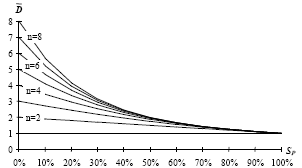
\includegraphics[scale=.6]{figura.png}}
\caption{Esta é a legenda da figura}
\label{fig:figura}
\end{figure}

\section{Conclusions}\label{sec:conclui}



%%English version: comment first, uncomment second
%\bibliographystyle{unsrt-pt}  % numeric, unsorted refs
\bibliographystyle{unsrt}  % numeric, unsorted refs
\bibliography{refs}

\end{multicols}

\end{document}
